\documentclass[a4paper,11pt]{article}
\usepackage{graphicx} %LaTeX package to import graphics
\graphicspath{{figures/}} %configuring the graphicx package
\usepackage{amsmath}% For the equation* environment

\title{My first document}
\date{\today}
\author{Román García Guill \thanks{Max Planck Institute Plasma Physics}}
% Reduce the margins of for the paper

\usepackage{graphicx}
\usepackage{amsmath}
\usepackage{listings}

\lstset{
  language=Python,
  basicstyle=\ttfamily\small,
  frame=single,
}

\begin{document}
 \maketitle
 \newpage

Some of the \textbf{greatest}
discoveries in \underline{science} 
were made by \textbf{\textit{accident}}.

\begin{figure}[h]
    \centering
    \includegraphics[width=0.90\textwidth]{CasaReal.jpg}
    \caption{Spanish Royal Familiy and Goverment officials.}
    \label{fig:FamiliaReal}
\end{figure}
 
As you can see in figure \ref{fig:FamiliaReal}, the function grows near the origin. 
This example is on page \pageref{fig:FamiliaReal}.
 
\begin{itemize}
  \item The individual entries are indicated with a black dot, a so-called bullet.
  \item The text in the entries may be of any length.
\end{itemize}
\begin{enumerate}
  \item This is the first entry in our list.
  \item The list numbers increase with each entry we add.
\end{enumerate}

In physics, the mass-energy equivalence is stated 
by the equation $E=mc^2$, discovered in 1905 by Albert Einstein.

The mass-energy equivalence is described by the famous equation
\[ E=mc^2 \] discovered in 1905 by Albert Einstein. 

In natural units ($c = 1$), the formula expresses the identity
\begin{equation}
E=m
\end{equation}

Subscripts in math mode are written as $a_b$ and superscripts are written as $a^b$. These can be combined and nested to write expressions such as

\[ T^{i_1 i_2 \dots i_p}_{j_1 j_2 \dots j_q} = T(x^{i_1},\dots,x^{i_p},e_{j_1},\dots,e_{j_q}) \]
 
We write integrals using $\int$ and fractions using $\frac{a}{b}$. Limits are placed on integrals using superscripts and subscripts:

\[ \int_0^1 \frac{dx}{e^x} =  \frac{e-1}{e} \]

Lower case Greek letters are written as $\omega$ $\delta$ etc. while upper case Greek letters are written as $\Omega$ $\Delta$.

Mathematical operators are prefixed with a backslash as $\sin(\beta)$, $\cos(\alpha)$, $\log(x)$ etc.


\section{First example}

The well-known Pythagorean theorem \(x^2 + y^2 = z^2\) was proved to be invalid for other exponents, meaning the next equation has no integer solutions for \(n>2\):

\[ x^n + y^n = z^n \]

\section{Second example}

This is a simple math expression \(\sqrt{x^2+1}\) inside text. 
And this is also the same: 
\begin{math}
\sqrt{x^2+1}
\end{math}
but by using another command.

This is a simple math expression without numbering
\[\sqrt{x^2+1}\] 
separated from text.

This is also the same:
\begin{displaymath}
\sqrt{x^2+1}
\end{displaymath}

\ldots and this:
\begin{equation*}
\sqrt{x^2+1}
\end{equation*}




%%%%%%%%%%%%%%%%%%%%%%%%%%%%%%%%%%%%%%%%%%%%%%%%%%%%%%%%%%%%%%%%%%%%%%%%%%%%%%%



\section{Introduction}

This is intended to be a short intro
:)


\section{Methodology}

This are the methods:

As seen in \cite{example_ref}, the methods used are:

- bla
- bla
- bla



\section{Resultados}

La solución numérica obtenida se muestra en la Fig.~\ref{fig:poisson}.

\begin{figure}[h]
  \centering
  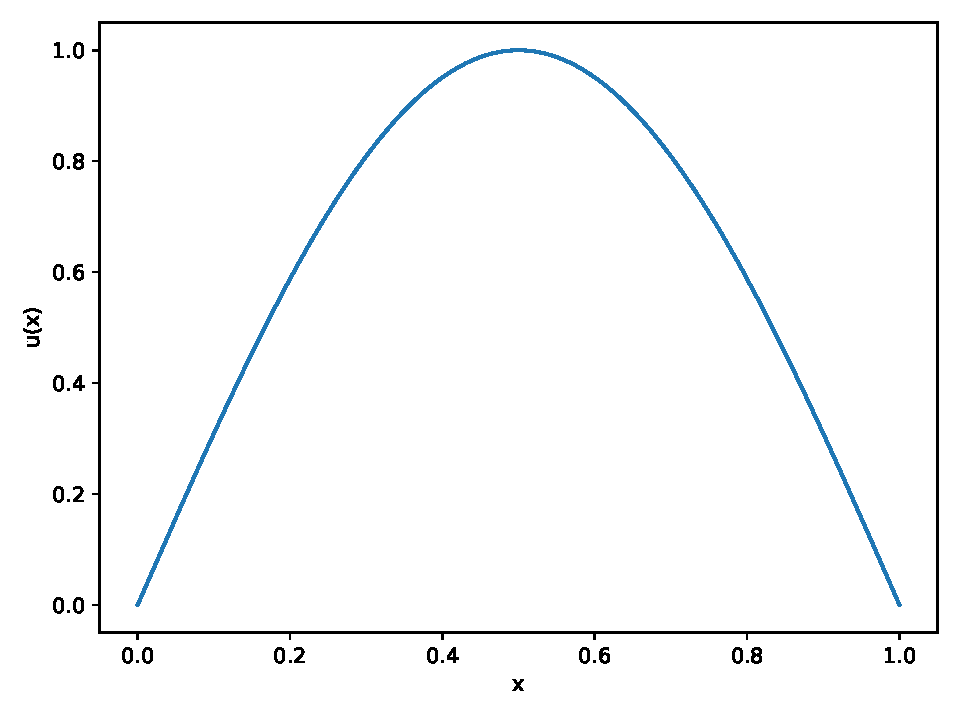
\includegraphics[width=0.65\textwidth]{figures/poisson.pdf}
  \caption{Solución numérica de la ecuación de Poisson en 1D.}
  \label{fig:poisson}
\end{figure}




\bibliographystyle{unsrt}
\bibliography{bibliography}

\end{document}
